\documentclass[conference]{IEEEtran}
\usepackage{amsmath,amssymb,amsfonts}
\usepackage{algorithmic}
\usepackage{graphicx}
\usepackage{textcomp}
\usepackage{xcolor}
\usepackage{biblatex}
\usepackage{titlesec}
\usepackage{float}
\usepackage{listings,xcolor}



\def\BibTeX{{\rm B\kern-.05em{\sc i\kern-.025em b}\kern-.08em
		T\kern-.1667em\lower.7ex\hbox{E}\kern-.125emX}}


\addbibresource{references.bib}

\begin{document}
	
	
	\title{Speaker Voice Similarity Analysis and Evaluation}
	
	
	\author{\IEEEauthorblockN{Carmel Gafa}
		\date{April 2025}
		
	}
	
	\maketitle
	
	\begin{abstract}
		This project investigates the effectiveness of the \texttt{WavLM-base-plus-sv} model for speaker voice similarity analysis using the Accents of the British Isles (ABI-1) corpus comprising 285 speakers across 14 regional accents. The study implements a fully automated pipeline that includes data cleansing, resampling, embedding extraction, and cosine similarity evaluation. Through intra- and inter-speaker comparisons, the model demonstrated high consistency within individual speakers and meaningful separability across speakers, especially those differing by gender or accent. A detailed threshold analysis was conducted using F1 score optimisation. Dimensionality reduction via Principal Component Analysis enabled visual exploration of embedding structure, while a K-Nearest Neighbours classifier was used to assess separability in the reduced space. The model effectively differentiated between phonetically distinct accents but showed reduced performance on similar regional dialects. These findings support the robustness of \texttt{WavLM} embeddings for speaker verification and highlight areas for refinement in accent-sensitive applications.
	\end{abstract}
	
	\section{Introduction}
	
	Speaker identification is the determination of a speaker's identity from a segment of their speech. It is crucial in applications such as personalised voice assistants, security systems, and partitioning audio streams according to each speaker's identity. Unlike speech recognition, which focuses on what is being said, speaker identification is concerned with who is speaking.
	
	This task can effectively be approached as a downstream application of pre-trained self-supervised speech models, such as \texttt{Wav2Vec2}\cite{baevski2020wav2vec} or its enhanced variant \texttt{WavLM}\cite{chen2022wavlm}. These models are trained on large-scale unlabelled audio datasets to learn audio representations that capture phonetic and speaker-specific characteristics.
	
	In this project, \texttt{WavLM-base-plus-sv}, a fine-tuned version of \texttt{WavLM} specialised for speaker verification, is used to extract speaker embeddings from audio samples. These embeddings are compared using cosine similarity to measure the similarity of two voice samples. This architecture enables a simple speaker identification pipeline without the need to train a model from scratch.
	
	
	\section{Data preprocessing}
	\label{sec:data-processing}
	
	The Accents of the British Isles (ABI) Corpus represents 13 regional accents. Figure \ref{fig:img-abi-corpus-accents} shows how these accents are categorised into four broad accent groups: Scottish, Irish, Northern English, and Southern English. Each broad group is further split into its respective regional accents~\cite{najafian2016improving}.
	
	\begin{figure}[H]
		\centering
		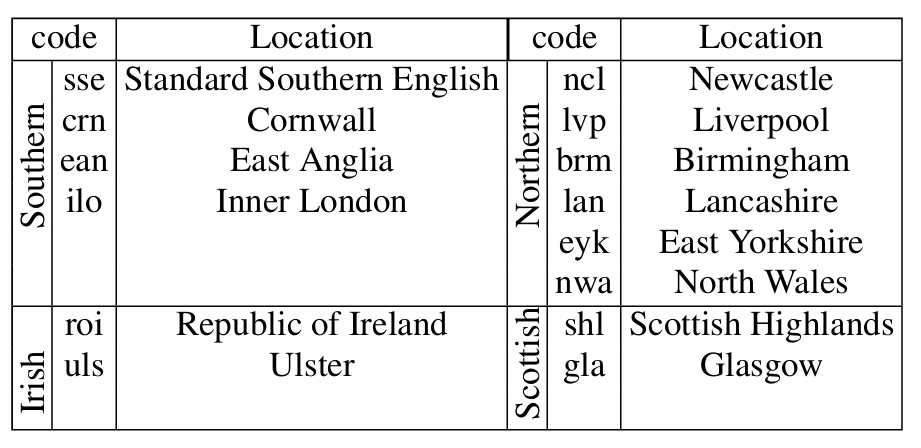
\includegraphics[width=0.7\linewidth]{img/img-abi-corpus-accents}
		\caption{List of accent codes and their corresponding geographical locations in the ABI-1 corpus~\cite{najafian2016improving}. The accents are grouped into four regional categories: Southern, Irish, Northern, and Scottish. This structure is used throughout the analysis to evaluate speaker similarity across and within regional accent groups.}
		\label{fig:img-abi-corpus-accents}
	\end{figure}
	
	The corpus includes 285 speakers, with speech collected from individuals who have lived in each regional accent area since birth. Each of the 285 subjects read the same three short passages. These short paragraphs form the 'sailor passage', with lengths of 92, 92, and 107 words with average durations of 43.2, 48.1, and 53.4 seconds, respectively~\cite{najafian2016improving}.
	
	The sources do not explicitly describe the recording conditions of the ABI corpus; however, it is mentioned that the speakers were selected by a phonetician, suggesting an effort for a standard quality recording for at least that accent~\cite{najafian2016improving}.
	
	\subsection{Signal resampling}
	\label{ssec:signal-resampling}
	
	Audio signals depend on two main parameters;
	
	\begin{itemize}
		\item number of channels $C$, that is $1$ for mono and $2$ for stereo.
		\item number of samples $T = t \times f_s$; that in turn depends on the
		\begin{itemize}
			\item duration $t$ of the audio in seconds.
			\item sampling rate $f_s$ (e.g. 48,000 Hz).
		\end{itemize}
	\end{itemize}
	
	For a mono signal, that is common in these applications, the utterance is stored in a vector that is then made available for processing,  $\mathbf{x}_{\text{raw}} \in \mathbb{R}^{1 \times T}$.
	
	The model by Microsoft that we are using in this example expects a signal rate of 16,000 Hz, and it is therefore necessary to resample the signal to this frequency. The resampling step involves selecting a subset of samples from the original vector, so that the original sampling rate $f_s^{\text{raw}}$ becomes a lower one $f_s^{\text{target}}$. The down-sampling ratio in this case, $R = \frac{f_s^{\text{raw}}}{f_s^{\text{target}}} = 3$
	
	Before reducing the number of samples, the high-frequency components from the original signals are removed, as they could cause aliasing. Aliasing occurs when frequencies above the new Nyquist frequency (one-half the new sampling rate) "fold back" into the signal, corrupting it. The Nyquist frequency after down-sampling becomes:
	
	$$f_N^{\text{new}} = \frac{f_s^{\text{target}}}{2} = 8000~\text{Hz}$$
	
	To remove the high frequency components, a low-pass filter is applied, generating a filtered signal, $\tilde{x}$
	
	$$\tilde{x}[n] = x_{raw}[n] * h[n]$$
	
	Where $h[n]$ is the impulse response of a low-pass filter, typically a windowed \texttt{sinc} function:
	
	$$h[n] = \text{sinc}\left(\frac{n}{R}\right) \cdot w[n]$$
	
	Here, $w[n]$ is a window function (like Kaiser, Hamming, etc.) to localise the infinite \texttt{sinc} filter in time.
	
	\begin{figure}[H]
		\centering
		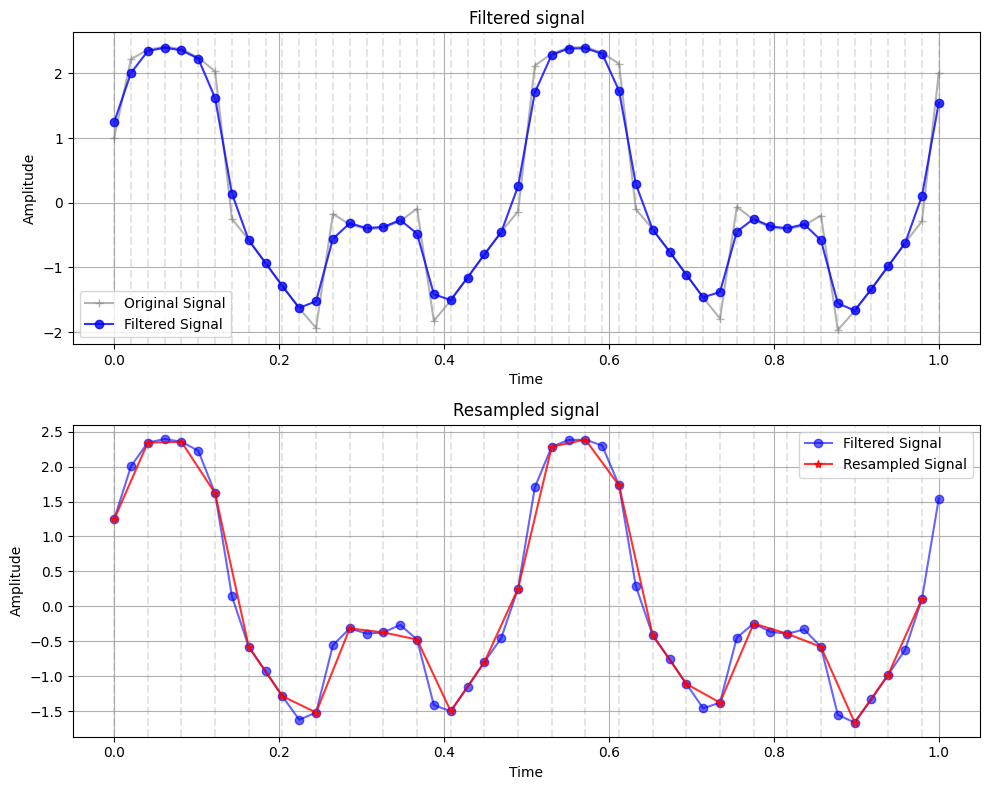
\includegraphics[width=0.9\linewidth]{img/img-resampling}
		\caption{Visualisation of the signal processing steps applied during audio preprocessing. The top plot shows the original and filtered signals, highlighting the smoothing effect of the filter. The bottom plot illustrates the effect of resampling the filtered signal to a target rate (e.g., 16\,kHz), with the resampled signal closely tracking the filtered one, preserving the original signal's structure while adjusting its temporal resolution.}
		\label{fig:img-resampling}
	\end{figure}
	
	If, as an example, we consider this function:
	
	\begin{align*}
		x_{raw} &=[x[0], x[1], x[2], x[3], x[4], x[5], x[6], x[7], x[8]]\\
		&=[2, 4, 6, 8, 10, 8, 6, 4, 2]
	\end{align*}
	
	and use the following windowed \texttt{sinc} filter (kernel)
	
	\begin{align*}
		h &= [h[0],\ h[1],\ h[2]]\\
		&= [0.2,\ 0.6,\ 0.2]
	\end{align*}
	
	We slide the kernel over the signal and compute:
	
	$$\tilde{x}[n] = \sum_{k=0}^{2} x[n + k] \cdot h[k]$$
	
	So that the first two samples of the filtered signal become;
	
	\begin{align*}
		\tilde{x}[0]	&= 0.2 \cdot x[0] + 0.6 \cdot x[1] + 0.2 \cdot x[2] \\
		&= 0.2\cdot2 + 0.6\cdot4 + 0.2\cdot6 \\
		&= 0.4 + 2.4 + 1.2 \\
		&= 4.0\\
		\tilde{x}[1] 	&= 0.2 \cdot x[1] + 0.6 \cdot x[2] + 0.2 \cdot x[3] \\
		&= 0.2\cdot4 + 0.6\cdot6 + 0.2\cdot8 \\
		&= 0.8 + 3.6 + 1.6 \\
		&= 6.0
	\end{align*}
	
	Once the signal is filtered, we can keep every $R^\text{th}$ sample and discard the rest (decimation), or apply interpolation to produce a smoother, resampled signal at the desired rate.
	
	$$x_{\downarrow R}[n] = x[Rn]$$
	
	So that, for example,
	
	$$x_{\downarrow 3}[n] = x[0], x[3], x[6], x[9], \dots$$
	
	\section{Methodology}
	
	In this section, we will discuss the implementation of the speaker voice similarity comparison pipeline. Several general criteria were observed during this exercise:
	
	\begin{itemize}
		\item Code that manipulated data was implemented in Python scripts, whereas code that analysed data was implemented in Python notebooks. This approach is preferred for several reasons:
		
		\begin{itemize}
			\item Scripts encourage modularity better.
			\item It is easier to import developed functions when using scripts.
			\item Scripts avoid the notebook's overheads like kernel restarts and variable state issues.
			\item The notebooks' interactive nature makes them very attractive for data analysis and tasks with a predominant visualisation component.
		\end{itemize}
		
		\item The analysis of voice similarity is broken down into discrete steps and implemented as stand-alone modules.    Each module will generate one or more results that are usually based on the results generated by previous modules in the pipeline. This approach is inspired by the medallion architecture, which is widely used in industry.
		\item Modules are stringed logically together to perform all the tasks necessary in this project, including the download of the data and model.
		\item Data is manipulated only using code. The whole project can be executed without any manual intervention whatsoever.
		\item Wherever possible, an option to execute the appropriate parts of a module on the GPU was made available.
		\item A simple logging tool was created so all modules can inject information about their execution. This logger is also used by a timer decorator that was created to measure the duration of the various modules of this project.
	\end{itemize}
	
	\subsection{Comparison strategy}
	\label{ssec:comparison-strategy}
	
	As discussed in Section \ref{sec:data-processing}, three audio files are available for each speaker in the ABI-1 dataset, which will be used to determine the similarity of any speaker to all other speakers in the dataset. The following approach is used to determine similarity in this exercise.
	\begin{itemize}
		\item Each audio file is compared with the other audio files for a given speaker, a total of $\binom{3}{2} = 3$ comparisons, and the minimum value is retained as the intra-comparison result.
		\item For every speaker combination in the dataset, each audio file of one speaker is compared to all the audio files of the other speaker, a total of nine comparisons, and the maximum value is retained as the inter-comparison result.
	\end{itemize}
	
	This approach will determine the thresholds and results that ensure maximum separation, as the minimum distance between intra- and inter-comparisons will be examined.
	
	\subsection{Voice similarity comparison pipeline}
	
	\begin{figure}[H]
		\centering
		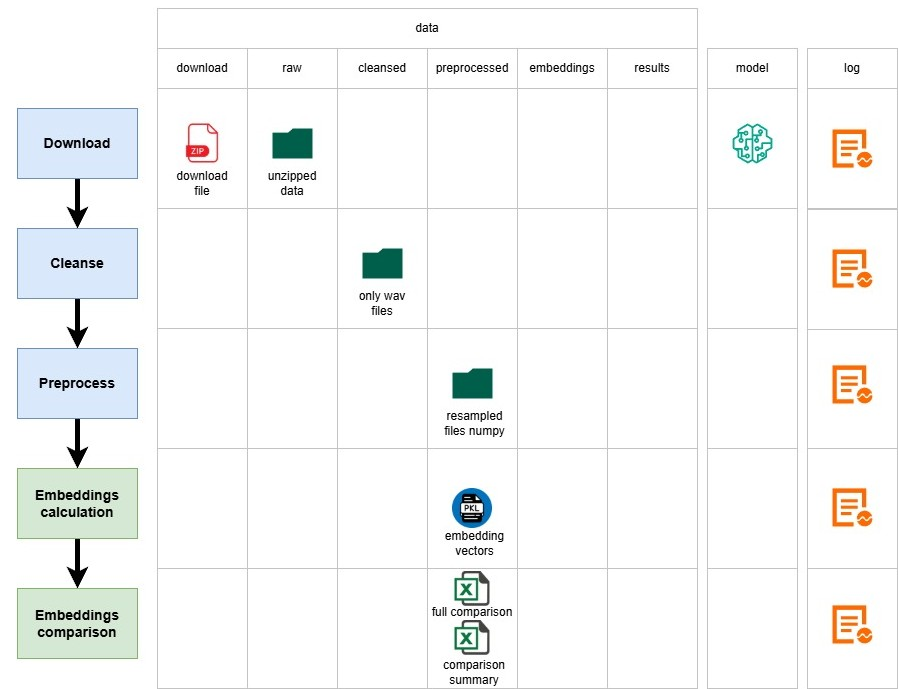
\includegraphics[width=1\linewidth]{img/img-pipeline}
		\caption{Overview of the speaker similarity analysis pipeline and associated file structure. Each processing stage—download, cleanse, preprocess, embeddings calculation, and embeddings comparison—produces outputs stored in dedicated folders. The flow diagram on the left outlines the logical sequence, while the table maps each module to its corresponding outputs across the \texttt{data}, \texttt{model}, and \texttt{log} directories.}	
		\label{fig:img-pipeline}
	\end{figure}
	
	Figure~\ref{fig:img-pipeline} shows the flow that was implemented as part of this project, which is made up of the following modules:
	
	\begin{itemize}
		\item \textbf{Download}. In the first step of the pipeline, the \texttt{ABI-1} dataset archive is downloaded and placed in the \texttt{data/download} folder. The contents are then extracted and placed in the \texttt{data/raw folder}. The \texttt{ABI-1} structure has an \texttt{accents/genders/speakers} configuration, whereby accents folders contain a male and female folder for each speaker. At this point, the data also contains additional data, such as transcription information.
		The \texttt{wavlm-base-plus-sv} model is also downloaded from Hugging Face using the \texttt{transformers} library and placed in the \texttt{model} folder.
		This module also contains the functionality to create the data, module and log folder structure necessary for this project.
		
		\item \textbf{Cleanse}. In the next step, the contents of each speaker, in each gender and each accent in the raw data folder, are examined, and only the files matching the pattern \texttt{shortpassage*.wav} are retained. The results are replicated in an identical folder structure in the \texttt{data/cleansed} folder.
		
		\item \textbf{Preprocess}. As discussed in Section~\ref{ssec:signal-resampling}, the audio files need to be preprocessed to 16 kHz using \texttt{torchaudio.transforms.Resample} so that the model can evaluate their embeddings. In this next step, all the audio files of each speaker, in each gender and accent, in the raw data folder are loaded and resampled. The resulting \texttt{numpy} arrays are stored in an identical folder structure in \texttt{data/preprocessed}.
		
		\item \textbf{Embedding calculation}. In the next step, the \texttt{wavlm-base-plus-sv} model calculates the embeddings for each audio data file. Each embedding is a 512-element vector, resulting in a $3 \times 512$ array for each speaker. The embedding information is stored in a dictionary data structure having "\texttt{accent-gender-speaker}" as key and the embedding array as the value during processing. It is then converted to a \texttt{pandas} \texttt{DataFrame} and saved as a pickle file in \texttt{data/embeddings}.
		
		\item \textbf{Comparison}. The final step of the pipeline implements pairwise cosine-similarity using the strategy explained in Section~\ref{ssec:comparison-strategy}. Two files are generated in this process:
		
		\begin{itemize}
			\item A raw results file containing the results of all comparisons: a set of three results for intra-comparison and a set of nine results for inter-comparison.
			\item A summary results file containing the selected comparison from each set using the strategy described previously.
		\end{itemize}
		
		The result files are stored in the \texttt{data/results} folder.
	\end{itemize}
	
	\section{Evaluation and results}
	\label{scn:evaluation-and-results}
	
	The analysis presented in this section was conducted using \texttt{analysis.ipynb} Jupyter notebook. The objective is to evaluate the performance of the \texttt{WavLM} model in a speaker similarity context. 
	This notebook is an important component in conjunction with the speaker similarity analysis pipeline, as it delivers insight into the separability of speaker embeddings and the robustness of the overall system.
	
	We start by examining the distributions of some of the groups in this system. 
	
	Figure~\ref{fig:img-self-similarity} presents a histogram showing the distribution of cosine similarity values obtained from intra-speaker comparisons, where, as described in Section~\ref{ssec:comparison-strategy}, each value in this plot represents the minimum similarity between two utterances from the same speaker. We can see that most of the same-speaker similarity scores fall within a high similarity range between approximately 0.985 and 0.997. 
	
	\begin{figure}[H]
		\centering
		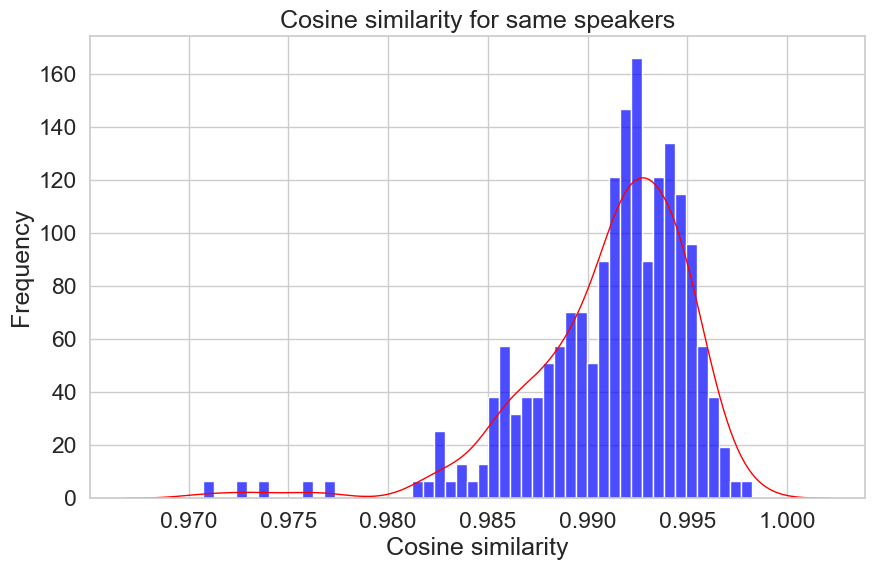
\includegraphics[width=0.7\linewidth]{img/img-self-similarity}
		\caption{Distribution of cosine similarity scores for same-speaker comparisons. The histogram shows a strong concentration of similarity values in the 0.985–0.997 range, indicating high consistency of embeddings produced by the \texttt{WavLM} model for recordings from the same speaker. A slight leftward tail suggests occasional variability due to acoustic or recording conditions.}
		\label{fig:img-self-similarity}
	\end{figure}
	
	As expected, these results are tightly concentrated around the upper bound of the cosine similarity scale, showing that the \texttt{WavLM} model produces highly consistent embeddings for recordings belonging to the same speaker. 
	
	The distribution also shows a small leftward tail, with a few similarity values extending up to 0.970. These lower outliers could be attributed to several factors, including acoustic variability across recordings, differences in speaking style or vocal effort, or background noise. It is important to reiterate that we are saving the minimum intra-similarity metric, and hence we are maintaining all low-scoring outliers without offsetting them with possibly better values. Nevertheless, the number of such occurrences is small relative to the whole dataset, and the core of the distribution remains strongly peaked at higher similarity values.
	
	Overall, we can conclude that this analysis confirms the robustness and discriminative power of the speaker embeddings generated by \texttt{WavLM} for intra-speaker comparison tasks, which is both expected and highly desirable.
	
	Next, we investigate the similarity of speakers of different genders, who should have the worst comparison scores, as the pitch difference is highly prevalent in this case. As we are also comparing speakers with different accents, factors like allophonic variation are also present in this comparison. Figure~\ref{fig:img-similarity} displays the distribution of cosine similarity scores computed between different speakers of different genders, so that each score represents the maximum similarity between utterances from two distinct male and female speakers.
	
	Unlike the tightly clustered same-speaker distribution shown in Figure~\ref{fig:img-self-similarity}, this distribution is broader and centred significantly lower on the cosine similarity scale. Most values fall between 0.55 and 0.85, with a peak around 0.72. This spread is expected, as embeddings from different speakers, particularly those differing in vocal pitch and timbre due to gender, are naturally more dissimilar.
	
	\begin{figure}[H]
		\centering
		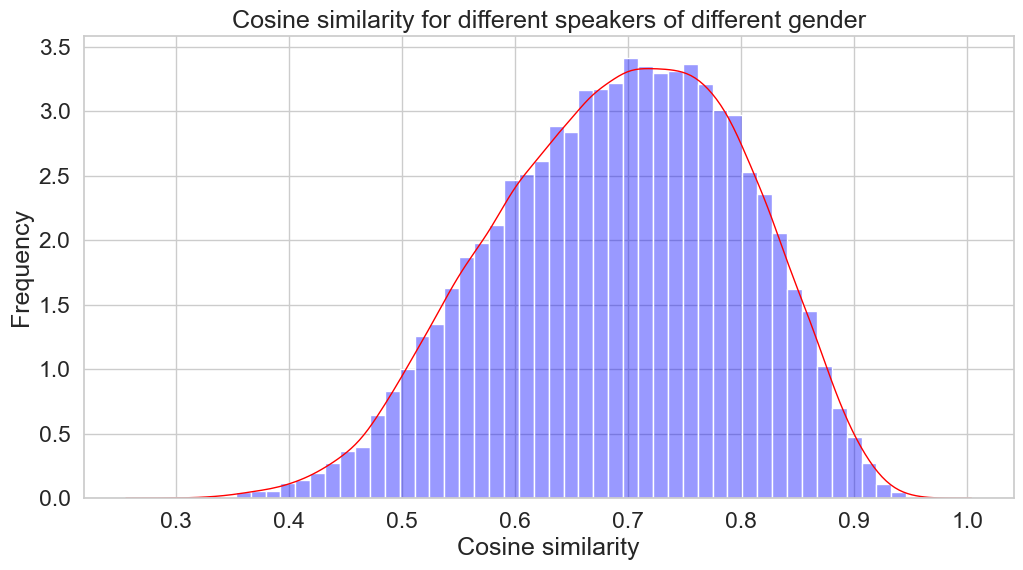
\includegraphics[width=0.7\linewidth]{img/img-similarity}
		\caption{Distribution of cosine similarity scores for different-speaker comparisons across genders. The histogram shows a wider and lower-centred distribution relative to same-speaker similarities, with most values ranging between 0.55 and 0.85.}
		\label{fig:img-similarity}
	\end{figure}
	
	The model demonstrates a good separation between same-speaker and different-gender-different-speaker comparisons. The minimal overlap between the lower tail of same-speaker scores observed in Figure~\ref{fig:img-self-similarity} and the upper tail of this distribution provides a practical rationale for selecting a threshold that effectively discriminates between same and different speakers.
	
	We finally examine the distributions of speakers of the same gender to appreciate the pitch's effect on cosine similarity. Although many factors weigh in on this result, we can presume that accent has some prevalence.
	
	\begin{figure}[H]
		\centering
		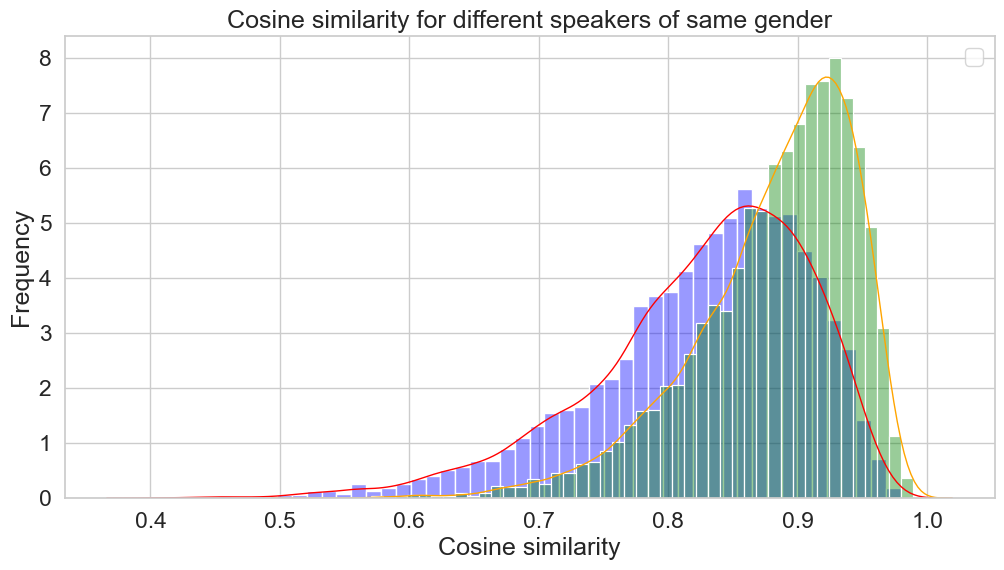
\includegraphics[width=0.7\linewidth]{img/img-similarity-same-gender}
		\caption{Distribution of cosine similarity scores for different-speaker comparisons within the same gender. The histogram distinguishes between male-male (blue) and female-female speaker pairs. Both distributions exhibit higher similarity values than cross-gender comparisons, with substantial overlap and peaks of 0.85 to 0.95.}	
		\label{fig:img-similarity-same-gender}
	\end{figure}
	
	Figure~\ref{fig:img-similarity-same-gender} illustrates the distribution of cosine similarity scores computed between speakers of the same gender, separated into male-male and female-female speaker pairings. Each value corresponds to the maximum similarity score observed among all utterance pairs between two distinct speakers within the same gender category.
	
	In contrast to the cross-gender distribution shown in Figure~\ref{fig:img-similarity}, male and female same-gender distributions are noticeably skewed toward higher similarity values. Most scores lie between 0.80 and 0.97, with both curves peaking at approximately 0.88 to 0.92. This increased similarity is likely due to shared vocal characteristics such as pitch range, speaking style, and formant patterns that are more common within the same gender group.
	
	While these distributions are distinguishable from same-speaker comparisons of Figure~\ref{fig:img-self-similarity}, they exhibit greater overlap with the same-speaker tail, particularly in the upper similarity range, presenting a more challenging case for threshold selection, as overly conservative thresholds may begin misclassifying some different-speaker pairs as same-speaker matches.
	
	\begin{figure}[H]
		\centering
		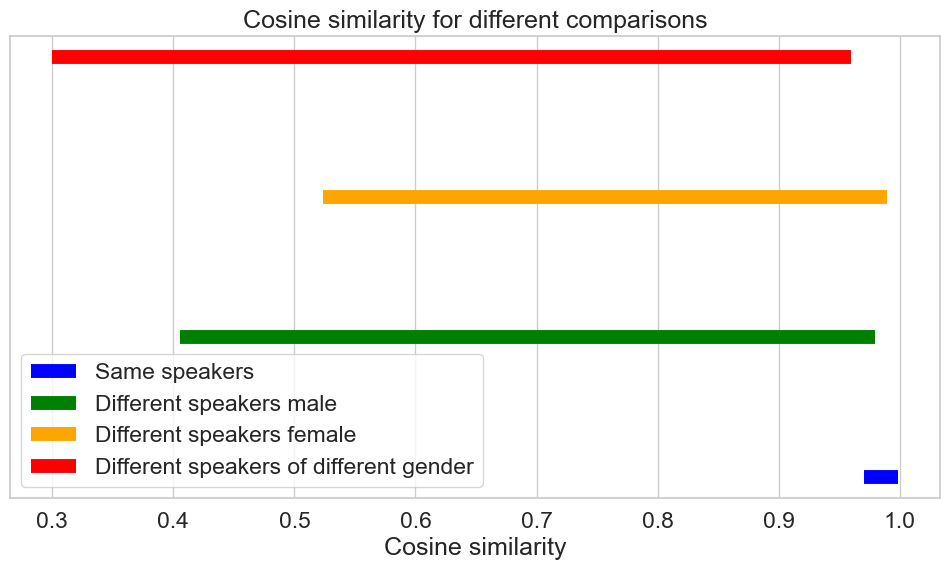
\includegraphics[width=0.7\linewidth]{img/img-similarity-comparison}
		\caption{Cosine similarity ranges across speaker comparison categories. Each horizontal bar represents the observed similarity range for a particular group: same-speaker pairs, different speakers of the same gender, and different speakers of different genders. This visual summary highlights the separation between intra- and inter-speaker similarities, supporting the choice of an effective threshold for speaker verification.}
		\label{fig:img-similarity-comparison}
	\end{figure}
	
	Figure~\ref{fig:img-similarity-comparison} summarises the cosine similarity ranges observed across all comparison categories analysed in the previous figures. Each horizontal bar illustrates the full range of similarity scores for a specific comparison group: same-speaker, male-male, female-female, and cross-gender pairs.
	
	The same-speaker scores form a narrow, high-range band, with values consistently close to 1.0. In contrast, all inter-speaker groups span broader ranges and are centred at lower similarity values. Cross-gender comparisons occupy the lowest band, typically ranging from 0.30 to 0.95, while same-gender comparisons show higher overlap with the same-speaker band, peaking near 0.90 or slightly above.
	
	This summary illustrates that while some overlap exists between same-speaker and same-gender-different-speaker comparisons, especially near the upper ends of the distributions, a significant gap exists that allows for a robust decision threshold definition.
	
	For this illustration, we can deduce that a well-chosen threshold, in the 0.95–0.98 range, can effectively separate same-speaker matches from different-speaker mismatches while minimising false acceptances and rejections.
	
	\subsection{Threshold selection}
	
	In the previous section, we noticed that the number of different-speaker pairs vastly exceeds that of same-speaker pairs, resulting in an insignificant imbalance in the dataset.
	
	In this case, traditional metrics such as accuracy can be misleading as a model biased toward predicting "different "speakers can still achieve high accuracy without performing well on identifying same-speaker pairs. 
	
	F1 score provides a more informative measure in this context,  as it captures the harmonic mean of precision and recall, thereby balancing the trade-off between false positives and false negatives. As we will see in this section, the F1 score remains low for most thresholds but exhibits a sharp peak at a specific value, indicating a precise point at which the model achieves its best balance of sensitivity and specificity. 
	
	
	\begin{figure}[H]
		\centering
		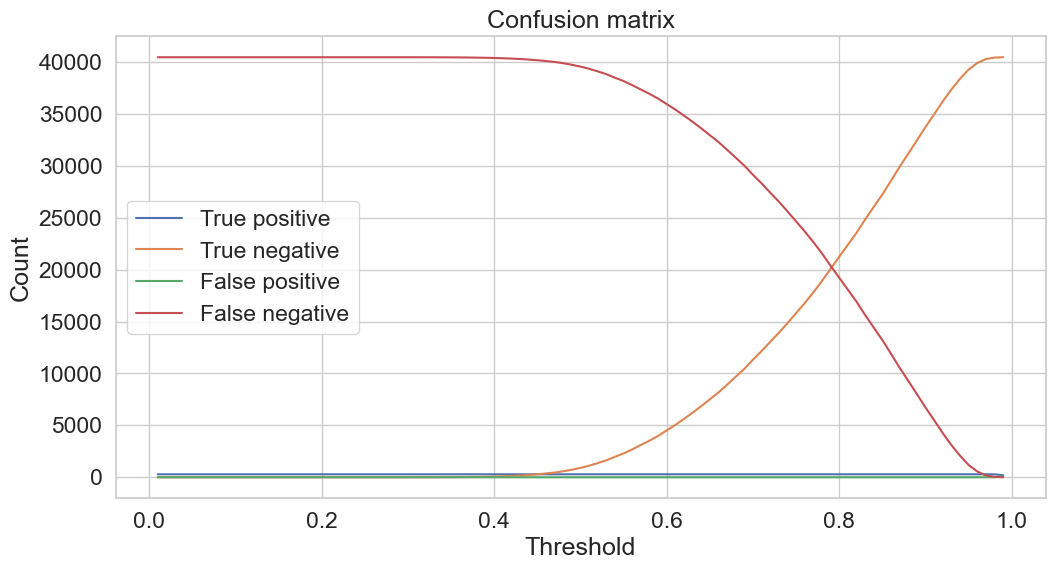
\includegraphics[width=0.7\linewidth]{img/img-confusion-matrix}
		\caption{Variation of confusion matrix components as a function of the similarity threshold. The plot shows how true positives, true negatives, false positives, and false negatives evolve as the decision boundary is adjusted. This visualisation aids in selecting a threshold that balances correct classification and error rates for speaker verification.}
		\label{fig:img-confusion-matrix}
	\end{figure}
	
	
	Figure~\ref{fig:img-confusion-matrix} illustrates how the components of the confusion matrix evolve as a function of the decision threshold applied to cosine similarity scores.
	
	This plot was generated using a threshold sweep and classifying speaker pairs as the same speaker if their similarity exceeds the current threshold.
	
	\begin{figure}[H]
		\centering
		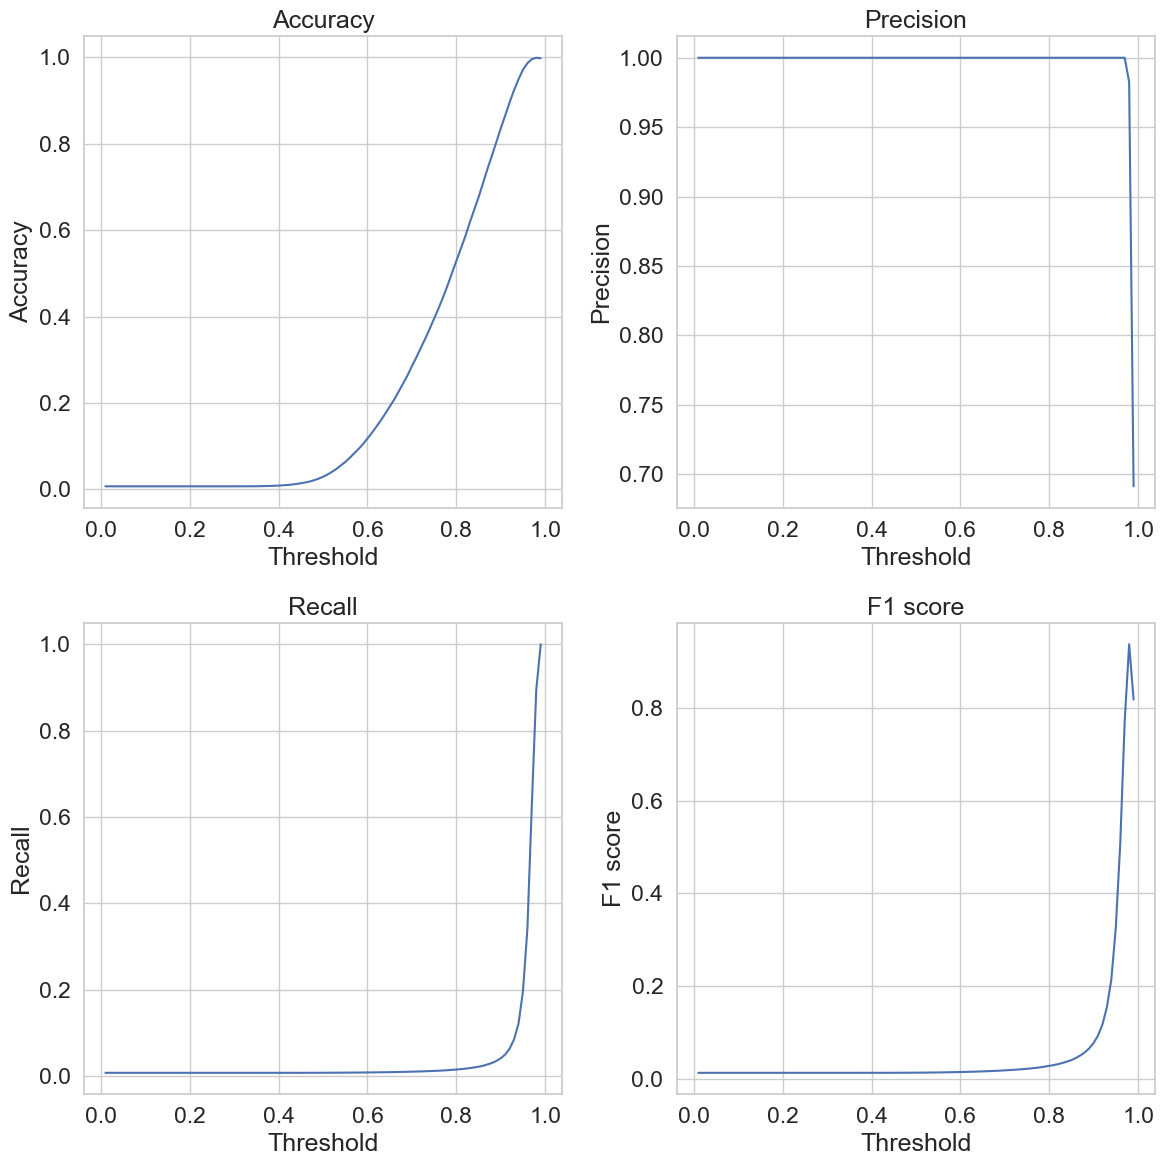
\includegraphics[width=0.9\linewidth]{img/img-metrics}
		\caption{Evaluation metrics as a function of the cosine similarity threshold. The plots show how accuracy, precision, recall, and F1 score evolve across thresholds ranging from 0 to 1. This analysis helps identify the optimal decision boundary that balances classification performance in an imbalanced speaker verification dataset.}
		\label{fig:img-metrics}
	\end{figure}
	
	The confusion matrix components were computed for each threshold value in the range [0.01, 1.00]. True positives represent correctly identified same-speaker pairs, while true negatives correspond to correctly rejected different-speaker pairs. False positives occur when different-speaker pairs are incorrectly classified as the same-speaker, and false negatives represent missed detections of same-speaker pairs.
	
	The results show, as expected, that at low thresholds, the model over-predicts same-speaker relationships, leading to high false positive and false negative counts. As the threshold increases, false positives decrease while false negatives increase. The true-negative count rises steadily with the threshold, whereas true positives remain relatively flat due to the limited number of same-speaker comparisons.
	
	Figure~\ref{fig:img-metrics} presents accuracy, precision, recall, and F1 score plotted as functions of the cosine similarity threshold. This analysis aims to identify the threshold that achieves the best trade-off between correctly identifying same-speaker pairs and avoiding false classifications.
	
	The accuracy curve shows a steep rise beginning around threshold 0.85, eventually approaching 1.0. However, given the imbalance in the dataset, accuracy alone is not a reliable metric. Precision remains nearly constant and close to 1.0 across all thresholds until a sharp drop near 1.0, indicating that when the model does predict a pair as same-speaker, it is almost always correct, though such predictions are rare.
	
	Recall values are close to zero across most thresholds and only increase sharply at the high end, suggesting that most same-speaker pairs are missed unless a very high threshold is applied. This behaviour is reflected in the F1 score, which stays low until it peaks abruptly at a threshold near 0.97–0.99, indicating a narrow window where precision and recall are reasonably balanced.
	
	These curves reinforce the importance of using the F1 score in threshold selection for imbalanced data. The optimal threshold corresponds to the peak of the F1 score curve, where the model achieves its best-combined performance in identifying same-speaker pairs while maintaining high precision. The maximum F1, calculated from this plot, had a value of \texttt{0.93645} and occurred at at threshold 0.98
	
	\section{Analysis and discussion}
	
	The results from Section~\ref{scn:evaluation-and-results} prove that the model can discriminate well but also reveal critical nuances that merit deeper investigation. The sharply concentrated distribution of same-speaker similarities indicates that the \texttt{WavLM} model reliably encodes speaker identity, producing consistent embeddings across multiple utterances.
	
	In contrast, the broader and more dispersed distributions for different-speaker pairs, particularly cross-gender comparisons, suggest that the model effectively captures inter-speaker variation. However, the analysis also shows that same-gender-different-speaker comparisons are less cleanly separated from same-speaker pairs, creating a zone of overlap that challenges perfect classification.
	
	The threshold analysis, where we examined confusion matrix components across a broad sweep of decision boundaries, highlights this overlap. 
	
	The system achieves excellent precision throughout most thresholds, but recall remains low until a very high threshold is applied, which is expected, as we have seen in Figure~\ref{fig:img-similarity-comparison}; the cosine similarity for the same speakers is concentrated in the higher values, and therefore, we need a high threshold to start eliminating the false negative values. The F1 score, which balances these competing objectives, peaks in a narrow band around 0.98, emphasising the system's sensitivity to small changes in the threshold. These findings demonstrate that while the core architecture performs well, the speaker verification pipeline is inherently sensitive to class imbalance and acoustic similarity within speaker groups. 
	
	Using cosine similarity as a decision metric works well in aggregate but cannot fully resolve confounding edge cases where inter-speaker similarity approximates intra-speaker variation, and therefore, a deeper exploration of the embedding space to understand what patterns, such as gender or accent, might be implicitly captured by the model, and where it might struggle. This section will use clustering analysis through dimensionality reduction to visualise speaker comparisons across similar and distant accents. We will also attempt to, very crudely, cluster this information and review the error achieved in such an operation.
	
	\subsection{Clustering analysis}
	
	In the previous sections, we discussed speaker voice similarity at length, and we built a robust speaker identification engine. Here, we will use clustering analysis to understand the structure of the embedding space produced by the speaker verification model. We will investigate whether the model captures patterns such as gender or accent.
	
	In this analysis, dimensionality reduction was carried out using Principal Component Analysis, which projected the high-dimensional embeddings into a two-dimensional space, allowing for visual inspection of potential clusters.
	
	A K-Nearest Neighbours classification was also implemented on the reduced-dimensionality data to evaluate how well the speaker embeddings preserve identity information, where embeddings projected via Principal Component Analysis are used as input features to a K-Nearest Neighbours classifier, with speaker accent (or identity) serving as the target label. We can use this method to assess how distinguishable speakers are in the reduced embedding space by training the classifier on a subset of embeddings and computing the training error. The K-Nearest Neighbours classification algorithm makes no assumptions about the underlying data distribution. It relies solely on distance metrics, aligning well with the cosine-based similarity framework used in our analysis. A low training error would confirm that the embedding space retains strong identity information even after dimensionality reduction.
	
	\subsubsection{Random speakers}
	
	We start with a very high-level cluster analysis, where Principal Component Analysis was carried out on a random embedding from 200 arbitrary speakers. This first analysis was conducted to get a feel for the scenario.
	
	\begin{figure}[H]
		\centering
		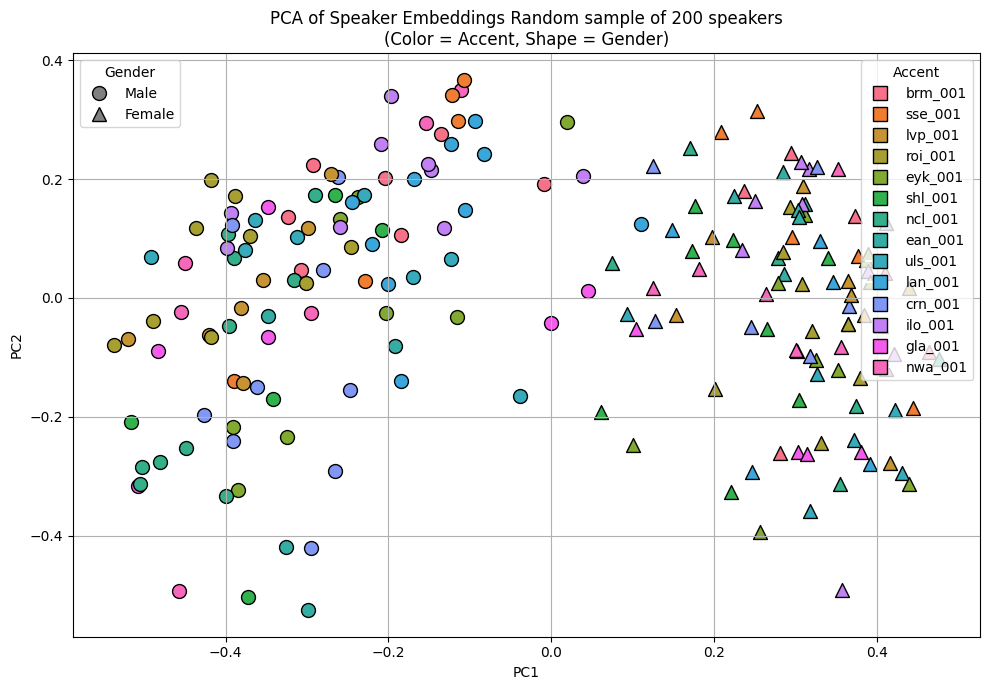
\includegraphics[width=0.7\linewidth]{img/img-cluster-all}
		\caption{Principal Component Analysis plot of speaker embeddings for 200 randomly selected speakers. Each point represents a speaker embedding, with the marker shape indicating gender and colour indicating accent group. The plot reveals a strong separation by gender along the first principal component, while accent-based clustering appears less distinct, with significant overlap among accent groups.}
		\label{fig:img-cluster-all}
	\end{figure}
	
	The resulting Principal Component Analysis is shown in Figure~\ref{fig:img-cluster-all}. It reveals a clear separation based on gender, where the first principal component strongly encodes gender-specific vocal features. 
	
	In contrast, accent-based clustering is far less distinct. The various accent groups appear heavily intermixed between both genders, indicating that accent information is not as prominently captured in the top two principal components. 
	
	We can therefore presume that to assess accent separability better, it may be necessary to restrict the analysis to a limited number of accents; although in some cases, this reduction might also be unfruitful. Overall, this visualisation demonstrates that while the model effectively captures gender characteristics, accent-related differences may be more subtle and require more targeted analysis.
	
	
	\subsubsection{Speakers from two distinct accents}
	
	We simplify our investigation of accent comparisons by limiting our analysis to accent pairs. This exercise examines how cleanly the clusters separate based on these two accent categories.
	
	We start by comparing  Scottish Highland (\texttt{shl\_001}) and Inner London (\texttt{ilo\_001}) accents as they offer a valuable test case for evaluating the accent sensitivity of the speaker embeddings. 
	
	\begin{figure}[H]
		\centering
		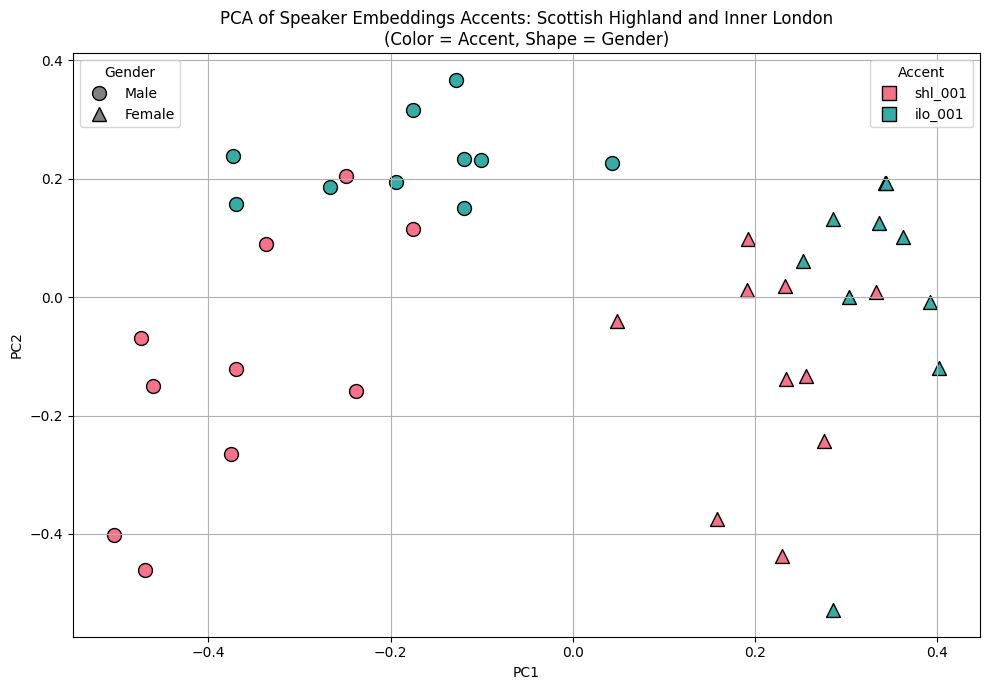
\includegraphics[width=0.7\linewidth]{img/img-cluster-shl-ilo}
		\caption{Principal Component Analysis plot of speaker embeddings for Scottish Highland and Inner London accents. Each point represents a speaker embedding, with marker shape indicating gender (circle for male, triangle for female) and colour representing accent. The visualisation reveals clear separability between the two accents along both principal components, suggesting that the model captures significant accentual differences between rural Scottish and urban London English.}
		\label{fig:img-cluster-shl-ilo}
	\end{figure}
	
	Apart from being significantly different in geography and sociolinguistic background, these accents are also phonetically distinct, making them suitable for testing whether the embedding space preserves regional phonetic variation.
	
	The resulting Principal Component Analysis plot, shown in Figure~\ref{fig:img-cluster-shl-ilo}, demonstrates a clear separation between the two accent groups across both principal components. Speakers from the Inner London group cluster toward the upper right side of the respective gender plot, while Scottish Highland speakers are concentrated on the lower left. This strong separability indicates that the model captures accentual variation effectively when the phonetic contrast between accent groups is significant. The separation persists across male and female speakers, suggesting that the accent features encoded in the embeddings are robust to gender variation.
	
	Figure~\ref{fig:knn-shl-ilo} illustrates the decision regions learned by a K-Nearest Neighbours classifier applied to speaker embeddings that were projected into two dimensions using Principal Component Analysis as described earlier. We notice that the classifier creates coherent decision regions around clusters of data points, indicating that the embedding space retains class-discriminative information even after dimensionality reduction. The relatively compact regions and minimal overlap between distinct classes suggest strong intra-speaker consistency and manageable inter-speaker variability.
	
	\begin{figure}[H]
		\centering
		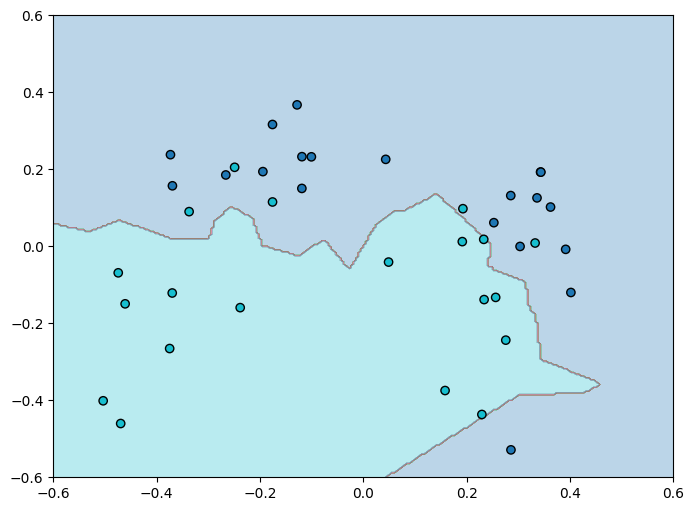
\includegraphics[width=0.7\linewidth]{img/img-knn-shl-ilo.png}
		\caption{Decision Boundary of K-Nearest Neighbours Classifier for this example.}
		\label{fig:knn-shl-ilo}
	\end{figure}
	
	The training error for this classification task is \textbf{12.5\%}, reinforcing that even a simple distance-based method like K-Nearest Neighbours classification can leverage the structural properties of the embedding space to achieve reasonable classification accuracy.
	
	\bigskip
	
	% reviewed
	
	Next, we compare speaker embeddings from the Birmingham (\texttt{brm\_001}) and Manchester (\texttt{lan\_001}) accent groups. These two urban Northern English accents share several phonetic and prosodic characteristics, including flattened intonation and similar vowel fronting, making them suitable for testing the model's sensitivity to subtle regional variation. 
	
	
	
	\begin{figure}[H]
		\centering
		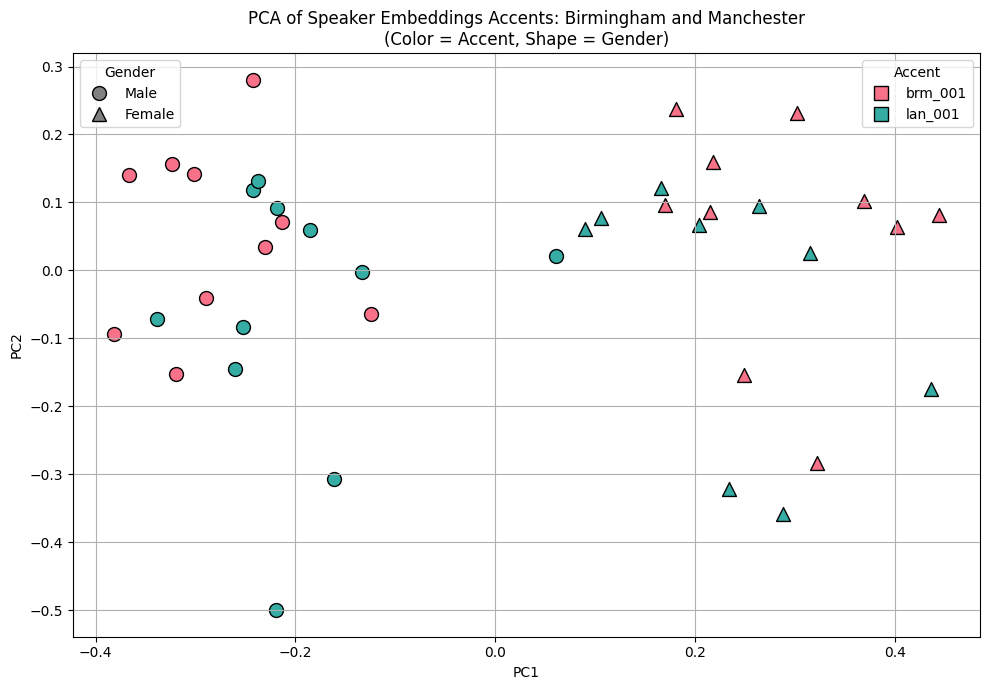
\includegraphics[width=0.7\linewidth]{img/img-cluster-brm-lan}
		\caption{Principal Component Analysis plot of speaker embeddings for Birmingham and Manchester  accents. Each point represents a speaker embedding, with marker shape indicating gender (circle for male, triangle for female) and colour representing accent. While some accent-based separation is visible, the overall clustering shows considerable overlap, particularly within gender groups, indicating that the model may not strongly distinguish between these two phonetically similar Northern English accents.}
		\label{fig:img-cluster-brm-lan}
	\end{figure}
	
	The Principal Component Analysis projection in Figure~\ref{fig:img-cluster-brm-lan} reveals some degree of separation between the accents along both principal components, with Manchester speakers more concentrated on the right and Birmingham speakers leaning toward the left. However, the clusters are not tightly bound, and there is significant overlap between the two groups, particularly within gender divisions, suggesting that while the model encodes some accentual information, it does not strongly distinguish between these two closely related dialects, especially when compared to more phonetically divergent pairs.
	
	\begin{figure}[h]
		\centering
		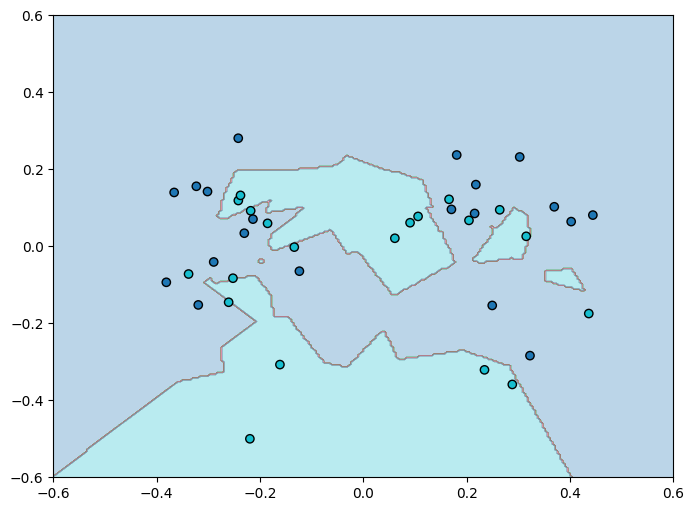
\includegraphics[width=0.7\linewidth]{img/img-knn-brm-lan.png}
		\caption{Decision Boundary of K-Nearest Neighbors Classifier on Speaker Embeddings from Birmingham (\texttt{brm\_001}) and Manchester (\texttt{lan\_001}).}
		\label{fig:knn-brm-lan}
	\end{figure}
	
	
	Figure~\ref{fig:knn-brm-lan} depicts the decision surface produced by a K-Nearest Neighbors classifier applied to speaker embeddings drawn from two closely related regional accents: Birmingham (\texttt{brm\_001}) and Manchester (\texttt{lan\_001}). The embeddings were first projected into two dimensions using Principal Component Analysis, and the classifier was trained to distinguish between the two accent groups.
	
	The resulting decision regions reveal a complex and fragmented landscape. Unlike cases involving phonetically distinct accents, the boundary shown here is highly non-linear and consists of disjoint regions that alternate between the two classes. This fragmentation suggests that the speaker embeddings for Birmingham and Manchester exhibit considerable overlap in the reduced space, making it difficult for the K-Nearest Neighbors classifier to form cohesive and contiguous class regions.
	
	This behavior is not unexpected. Both accents belong to the broader category of Northern English dialects and share a number of prosodic and phonetic traits. As a result, the model's embeddings for these speakers tend to occupy similar regions in the feature space. When projected to two dimensions, the separation becomes even less pronounced, and the K-Nearest Neighbors classifier—which relies solely on local distance-based decisions—responds by constructing highly localised decision zones.
	
	The scattered nature of the boundary thus reflects the limited discriminative power between these two accents under dimensional compression, and it underscores the difficulty of distinguishing between subtle regional variations using distance-based methods alone. This result aligns with prior observations in the clustering analysis and provides further evidence that accent separability is highly dependent on the magnitude of phonetic differences.
	
	
	
	
	
	
	\bigskip
	
	
	
	\subsubsection{Speaker separation}
	This investigation samples multiple utterances per speaker, focusing on 5 speakers. The analysis verifies intra-speaker consistency in embeddings, and whether utterances from the same speaker form tightly bound clusters regardless of content.
	
	
	
	\begin{figure}[h]
		\centering
		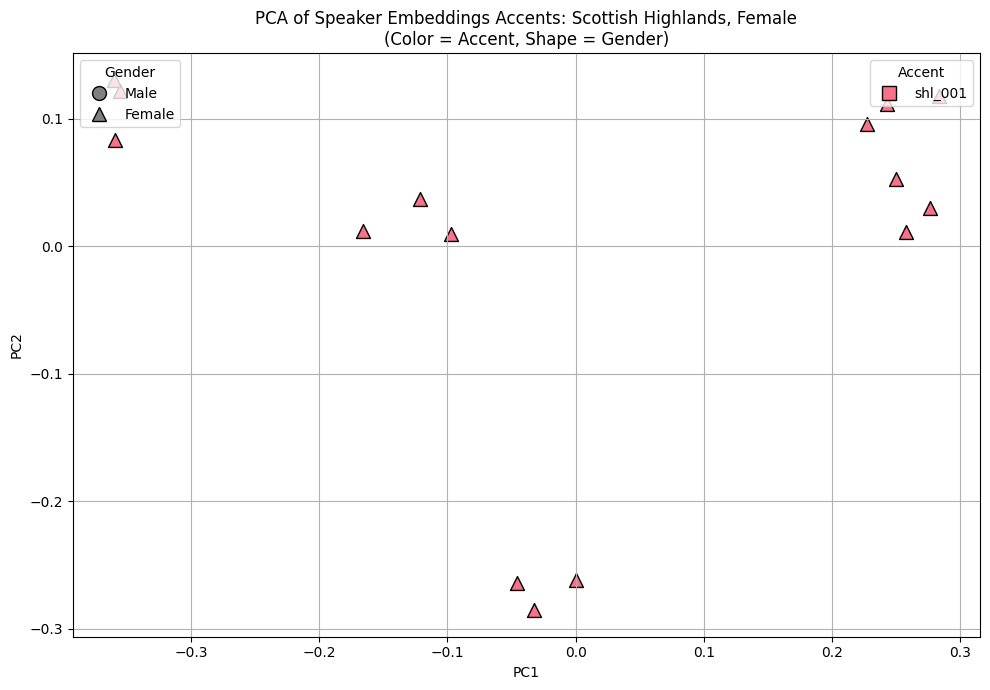
\includegraphics[width=0.85\linewidth]{img/img-cluster-speaker-separation.png}
		\caption{Principal Component Analysis of Speaker Embeddings for Scottish Highlands, Female Speakers. Each triangle represents one of the three utterance embeddings per speaker, projected onto the first two principal components.}
		\label{fig:pca-shl-female}
	\end{figure}
	
	
	Figure~\ref{fig:pca-shl-female} presents the result of applying Principal Component Analysis to the speaker embeddings of female speakers from the Scottish Highlands accent group (\texttt{shl\_001}). Each speaker in this subset contributed three utterances, resulting in three embeddings per speaker. These embeddings were projected into two dimensions using the first two principal components, and each triangle in the plot corresponds to one of these projected embeddings.
	
	The visualisation reveals that for most speakers, the three embeddings lie in close proximity to one another, forming compact clusters. This behavior indicates a high degree of consistency in the representation of speaker identity across different utterances, even though the utterances may vary slightly in content, duration, or prosodic variation. The tight grouping of each speaker's embeddings supports the effectiveness of the WavLM model in generating stable and speaker-specific representations.
	
	Moreover, the spread of the clusters across the plot shows clear between-speaker variability, suggesting that the model can distinguish among different speakers, even within the same accent and gender group. This result reinforces earlier findings that WavLM embeddings are highly discriminative and preserve speaker-specific features, making them suitable for downstream tasks such as speaker verification or diarization.
	
	\begin{figure}[h]
		\centering
		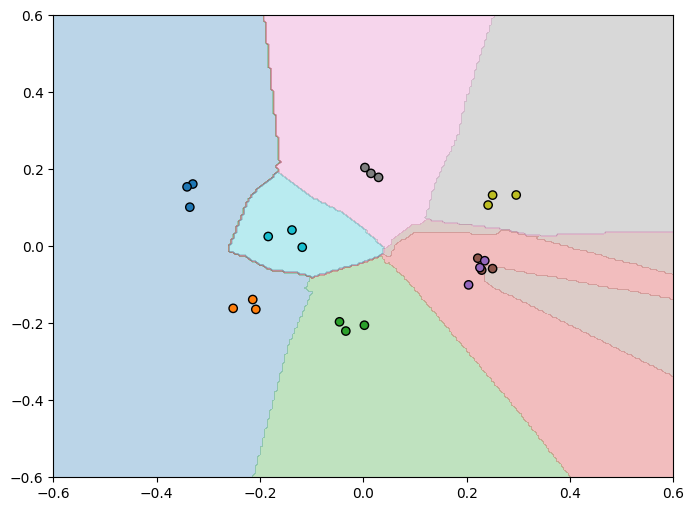
\includegraphics[width=0.7\linewidth]{img/img-knn-speaker-separation.png}
		\caption{Decision Boundaries of K-Nearest Neighbors Classifier for Multiple Speakers. Each point corresponds to a single utterance embedding projected via Principal Component Analysis. Background regions represent classification zones determined by the K-Nearest Neighbors algorithm.}
		\label{fig:knn-speaker}
	\end{figure}
	
	
	Figure~\ref{fig:knn-speaker} illustrates the classification boundaries generated by a K-Nearest Neighbors classifier trained on speaker embeddings from several speakers, with each speaker represented by multiple utterance samples. The embeddings were reduced to two dimensions using Principal Component Analysis for visualisation purposes, and each dot in the plot corresponds to an individual utterance. Distinct colors indicate different speaker labels, while the shaded background regions show the classifier's predicted zones.
	
	The visualised decision boundaries highlight a key strength of the K-Nearest Neighbors approach: its responsiveness to local data structure. In this figure, the classifier has effectively partitioned the space into distinct regions around clusters of utterances belonging to individual speakers. These clusters appear well separated, with each group residing predominantly within its own classification zone. This strongly suggests that the WavLM embeddings contain sufficient speaker-specific information, and that dimensionality reduction has preserved this structure to a meaningful extent.
	
	The irregular shape of some boundary regions reflects the instance-based nature of K-Nearest Neighbors, which makes no global assumptions about the data distribution. Despite this, the classifier demonstrates robust performance, producing largely clean separations between speakers.
	
	This visualisation confirms that even when multiple speakers are included, and despite the compression to two dimensions, the embedding space remains structured in a way that allows a simple, non-parametric classifier to reliably distinguish between individuals. It supports the broader conclusion that WavLM embeddings are both consistent and discriminative at the speaker level.
	
	
	
	\section{Conclusion and future work}
	
	
	
	This study evaluated the speaker similarity capabilities of the WavLM-base-plus-sv model using the ABI-1 corpus. The model demonstrated high intra-speaker consistency and clear separability from different-speaker embeddings through a detailed analysis of cosine similarity metrics between speaker embeddings, especially in cross-gender cases. Threshold tuning using F1 score optimisation further highlighted the system's robustness when carefully calibrated.
	
	The methodology incorporated a comprehensive preprocessing pipeline, cosine similarity-based evaluation, and dimensionality reduction via Principal Component Analysis. Embedding structures were further assessed through visual clustering and classification using K-Nearest Neighbors. The model exhibited reliable performance in differentiating phonetically distinct accents (e.g., Scottish Highland vs. Inner London), while accent pairs with high phonetic similarity (e.g., Birmingham and Manchester) proved more challenging, indicating areas where model refinement may be beneficial.
	
	Future work could explore the integration of alternative embedding aggregation techniques such as attention-based pooling, and dimensionality reduction methods like t-SNE or UMAP for non-linear structure preservation. Additionally, evaluating WavLM in comparison with other pre-trained models (e.g., ECAPA-TDNN or HuBERT) and in real-time inference contexts could further validate its applicability to speaker diarization and verification pipelines. The insights derived from this study affirm WavLM's effectiveness in speaker similarity tasks and pave the way for more adaptive, accent-aware speaker identification systems.
	
	\section*{Generative AI}
	
	\printbibliography
	
	
	
\end{document}
